\documentclass[border=4pt]{standalone}
% Shared style for FORGE paper figures (standalone, vector PDF)
\usepackage[T1]{fontenc}
\usepackage{lmodern}      % Latin Modern sans serif for diagrams
\renewcommand{\familydefault}{\sfdefault}
\usepackage{microtype}
\DisableLigatures[-]{encoding=T1,family=tt*}  % keep -- as two hyphens in CLI flags
\usepackage{textcomp}
\usepackage{amsmath}
\usepackage{tikz}
\usetikzlibrary{arrows.meta,positioning,calc,fit,backgrounds,shapes.geometric,shapes.misc,decorations.pathreplacing}

% ---- Moderate accent palette -------------------------------------------------
\definecolor{ink}{HTML}{222831}        % near-black text/borders
\definecolor{subink}{HTML}{5B6470}     % secondary text
\definecolor{accInput}{HTML}{2F5C9E}   % blue  -> plugin inputs
\definecolor{accModel}{HTML}{2A9D8F}   % teal  -> validated model / core
\definecolor{accGen}{HTML}{D7892B}     % amber -> generators / outputs
\definecolor{accVerif}{HTML}{6A4C93}   % purple-> verification
\definecolor{accMuted}{HTML}{8A94A3}   % grey  -> not-exercised / external

\colorlet{fillInput}{accInput!10}
\colorlet{fillModel}{accModel!14}
\colorlet{fillGen}{accGen!14}
\colorlet{fillVerif}{accVerif!12}
\colorlet{fillMuted}{accMuted!14}
\colorlet{fillPlain}{black!4}

% ---- Node styles -------------------------------------------------------------
\tikzset{
  font=\sffamily,
  >={Stealth[length=2.6mm,width=2.0mm]},
  base/.style={
    rounded corners=2pt, draw, line width=0.7pt,
    align=center, inner sep=5pt, text=ink,
    minimum height=10mm, font=\small},
  inbox/.style   ={base, draw=accInput, fill=fillInput},
  modelbox/.style={base, draw=accModel, fill=fillModel, line width=1.0pt},
  genbox/.style  ={base, draw=accGen,   fill=fillGen},
  verbox/.style  ={base, draw=accVerif, fill=fillVerif},
  mutedbox/.style={base, draw=accMuted, fill=fillMuted, text=subink},
  outbox/.style  ={base, draw=ink!55,   fill=fillPlain},
  title/.style   ={font=\bfseries\small, text=ink},
  grouptitle/.style={font=\bfseries\footnotesize, text=#1},
  lbl/.style     ={font=\scriptsize, text=subink, inner sep=2pt},
  flow/.style    ={draw=ink!70, line width=0.9pt, ->},
  flowmuted/.style={draw=accMuted, line width=0.8pt, ->, densely dashed},
  flowmodel/.style={draw=accModel, line width=1.1pt, ->},
  groupbg/.style ={rounded corners=4pt, draw=#1!55, line width=0.7pt,
                   fill=#1!5, dash pattern=on 3pt off 2pt},
}

\usetikzlibrary{patterns}
% Cycle counts of the vision platform-wrapper design: module latencies from
% data/platform_wrapper.forge.dot (norm 3, winbld 10, sobel 4, threshcfg 2, tstats 1,
% fixed delay 12) and tbnd's bounded latency of 1 to 17 cycles; arrivals at the merge
% points (17 and 17; 4..20 and 4) as in ../evidence/artifacts/latency_check_platform_wrapper.md.
\begin{document}
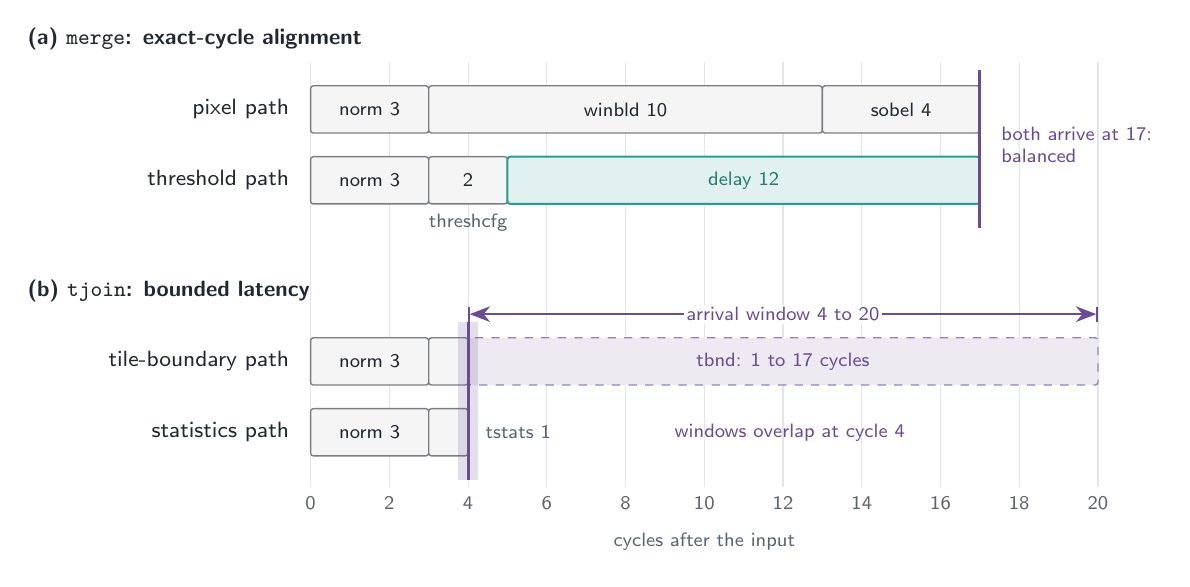
\begin{tikzpicture}[x=5mm, y=1mm,
  seg/.style={draw=ink!60, fill=fillPlain, line width=0.5pt, rounded corners=1pt},
  dly/.style={draw=accModel, fill=fillModel, line width=0.7pt, rounded corners=1pt},
  bnd/.style={draw=accVerif!70, fill=fillVerif, line width=0.5pt, dashed, rounded corners=1pt},
  sl/.style={font=\scriptsize, text=ink},
  rl/.style={font=\footnotesize, text=ink, anchor=east},
  pt/.style={font=\bfseries\footnotesize, text=ink, anchor=south west, inner sep=0pt},
]
\def\h{6}   % bar height (mm)

% ---- axis and grid, shared by both panels --------------------------------------------
\foreach \c in {0,2,...,20} {
  \draw[ink!12, line width=0.4pt] (\c,-45) -- (\c,9);
  \node[font=\scriptsize, text=subink, below] at (\c,-45) {\c};
}
\node[font=\scriptsize, text=subink, anchor=north] at (10,-49.5) {cycles after the input};

% ---- (a) exact-cycle merge at merge ------------------------------------------------------
\node[pt] at (-7.2,10.5) {(a) \texttt{merge}: exact-cycle alignment};
\node[rl] at (-0.3,3) {pixel path};
\draw[seg] (0,0) rectangle node[sl]{norm 3} (3,\h);
\draw[seg] (3,0) rectangle node[sl]{winbld 10} (13,\h);
\draw[seg] (13,0) rectangle node[sl]{sobel 4} (17,\h);
\node[rl] at (-0.3,-6) {threshold path};
\draw[seg] (0,-9) rectangle node[sl]{norm 3} (3,-9+\h);
\draw[seg] (3,-9) rectangle node[sl]{2} (5,-9+\h);
\draw[dly] (5,-9) rectangle node[sl, text=accModel!80!black]{delay 12} (17,-9+\h);
\node[font=\scriptsize, text=subink, anchor=north] at (4,-9) {threshcfg};
\draw[accVerif, line width=1.1pt] (17,-12) -- (17,8);
\node[font=\scriptsize, text=accVerif, anchor=west, align=left] at (17.3,-1.5)
  {both arrive at 17:\\balanced};

% ---- (b) bounded skew at tjoin -----------------------------------------------------------
\node[pt] at (-7.2,-21.5) {(b) \texttt{tjoin}: bounded latency};
\node[rl] at (-0.3,-29) {tile-boundary path};
\draw[seg] (0,-32) rectangle node[sl]{norm 3} (3,-32+\h);
\draw[seg] (3,-32) rectangle (4,-32+\h);
\draw[bnd] (4,-32) rectangle node[sl, text=accVerif]{tbnd: 1 to 17 cycles} (20,-32+\h);
\node[rl] at (-0.3,-38) {statistics path};
\draw[seg] (0,-41) rectangle node[sl]{norm 3} (3,-41+\h);
\draw[seg] (3,-41) rectangle (4,-41+\h);
\node[font=\scriptsize, text=subink, anchor=west] at (4.2,-38) {tstats 1};
\fill[accVerif, opacity=0.18] (3.75,-44) rectangle (4.25,-24);
\draw[accVerif, line width=1.1pt] (4,-44) -- (4,-24);
\draw[accVerif, line width=0.6pt, |<->|] (4,-23) -- node[font=\scriptsize, fill=white, inner sep=1pt, text=accVerif]{arrival window 4 to 20} (20,-23);
\node[font=\scriptsize, text=accVerif, anchor=west, align=left] at (9,-38)
  {windows overlap at cycle 4};

\end{tikzpicture}
\end{document}
